\chapter{Auswertung}
\label{sec:auswertung}

In diesem Abschnitt wollen wir nun verschiedene Resultate des Projekts IT-Jobs\index{IT-Jobs-Projekt} im Bezug auf Code-Qualität untersuchen und vergleichen.

Zuerst werden verschiedene Metriken, die im Verlauf der Entwicklung regelmäßig festgehalten wurden, näher betrachten. Im weiteren Teil vergleichen wir die erreichten Maßzahlen mit denen früherer Projekte der pludoni GmbH und einiger bekannter OpenSource Ruby-Projekte, um die Ergebnisse besser einordnen zu können.


\section{Entwicklungsstand IT-Jobs}
Zum Zeitpunkt der Beendigung dieser Arbeit sind folgende Teilmodule abgeschlossen:
\begin{itemize}
 \item Modul \glossar{CMS}: Blog und statische Seiten sowie die Möglichkeit variablen Inhalt auf beliebigen Seiten innerhalb der Sidebar darzustellen
 \item Modul Job, Basis: Implementation des Datenbank\index{Datenbank}schemas für Jobs und die Möglichkeit Jobs über das Interface anzulegen.
 \item Modul Feedimport: Möglichkeit, Jobs mittels einer XML-Schnittstelle in das System einzuspielen und E-Mail-Benachrichtigung im Falle eines Fehlers an den Inhaber der XML-Feeds.
\end{itemize}
Noch offen für eine zukünftige Entwicklung sind:
\begin{itemize}
 \item Modul: Bewerbung. Bewerber können sich über die Webseite bewerben. Ebenfalls können sie sich mit Facebook und LinkedIn verbinden, um automatisch ihre Stammdaten eintragen zu lassen
 \item Modul: Bezahlsystem: Beim Anlegen eines Jobs wird der Bezahlvorgang über einen externen Dienstleister abgewickelt.
\end{itemize}

Während der Arbeiten an IT-Jobs\index{IT-Jobs-Projekt} wurden andere Aufgaben priorisiert und deswegen der Abgabetermin für das System nach 2012 verlegt. Nichtsdestotrotz soll IT-Jobs als Basistechnologie und Referenzprojekt für weitere Rails\index{Ruby-on-Rails}-Anwendungen dienen und die Entwicklung kann insgesamt als Erfolg bewertet werden, auch wenn sie zum gegenwärtigen Zeitpunkt noch nicht abgeschlossen ist.

An der Entwicklung waren einschließlich des Autors zwei Programmierer beteiligt. Beiden Programmierern gelang es, sich mit der Testgetriebene\index{TDD}n Entwicklung und mit Rails\index{Ruby-on-Rails} vertraut zu machen und wertvolle Erfahrungen zu sammeln.

\subsection*{Code-Qualität und Testabdeckung}
Während der Entwicklung wurden in regelmäßigen Abständen Code-Metrik\index{Code-Metrik}en festgehalten und können nun so über den Verlauf der Entwicklung dargestellt werden.

\begin{figure}[htbp]
 \centering
 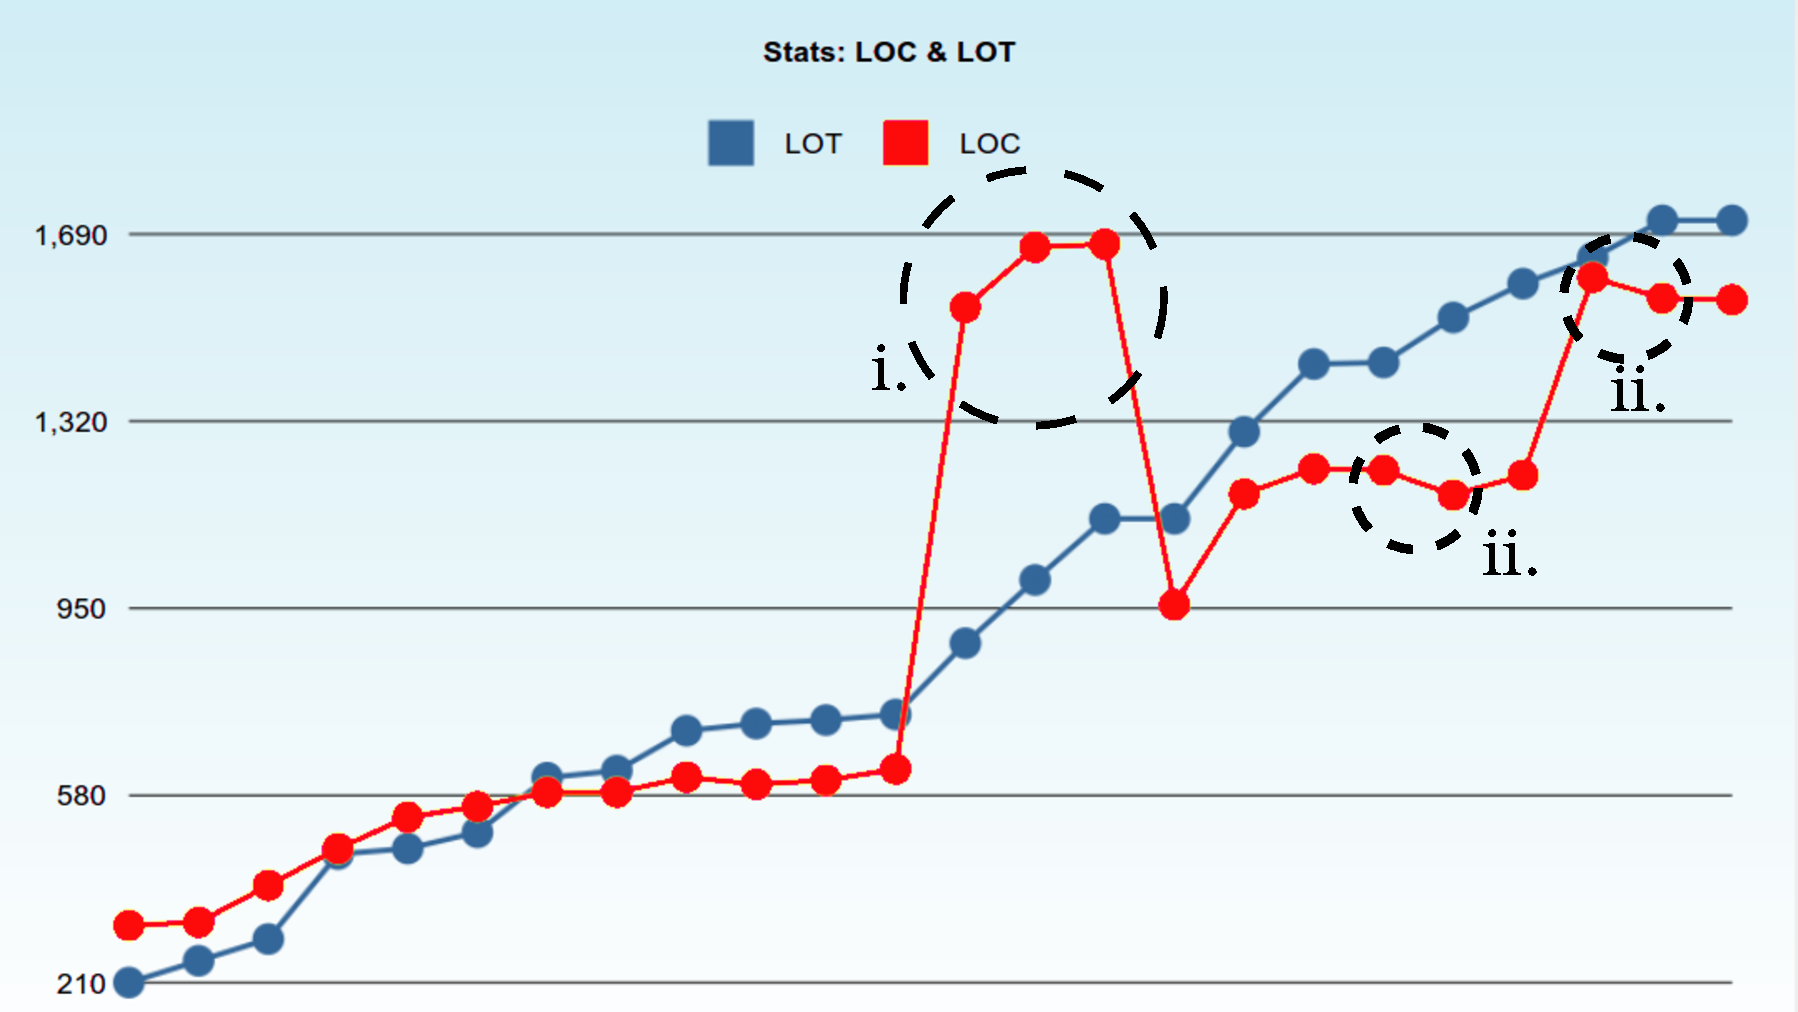
\includegraphics[width=0.9\textwidth]{./diagrams/itjobs-loclot.pdf}
 % itjobs-loclot.png: 1000x600 pixel, 72dpi, 35.28x21.17 cm, bb=0 0 1000 600
 \caption{Entwicklung des Umfangs des Test- und Programmcodes}
 \label{fig:itjobsLoc}
\end{figure}

In Abbildung \ref{fig:itjobsLoc} ist der Verlauf der Codezeilen und der Testzeilen abgebildet. Während in den ersten Tagen der Entwicklung, wegen des Einsatzes von Codegenerator\index{Code-Generator}en und einer langsamen Gewöhnung an den TDD\index{TDD} Ablauf, noch weniger Testcode als Programmcode geschrieben wurde, verlaufen die Linien ab dann nahezu proportional. Einen Ausreißer stellen die mit i. markierte Codezeilen dar: Hier ist eine Fehlkonfiguration der Statistikberechnung die Ursache dafür, dass Fremdcode mitgezählt wurde, der nicht Teil der Anwendung war. Eine andere interessante Erkenntnis ist, dass zwar die Lines Of Test \index{Test}monoton steigend ist, die Lines Of Code dagegen durch Refaktorisierung\index{Refaktorisierung}en abgefallen sind (z.B. mit ii. markierte Stellen). Die hohe Testdichte hat eine Refaktorisierung ermöglicht und in diesen Phasen konnte effektiv Design zu dem System hinzugefügt werden.


\begin{figure}[htbp]
 \centering
 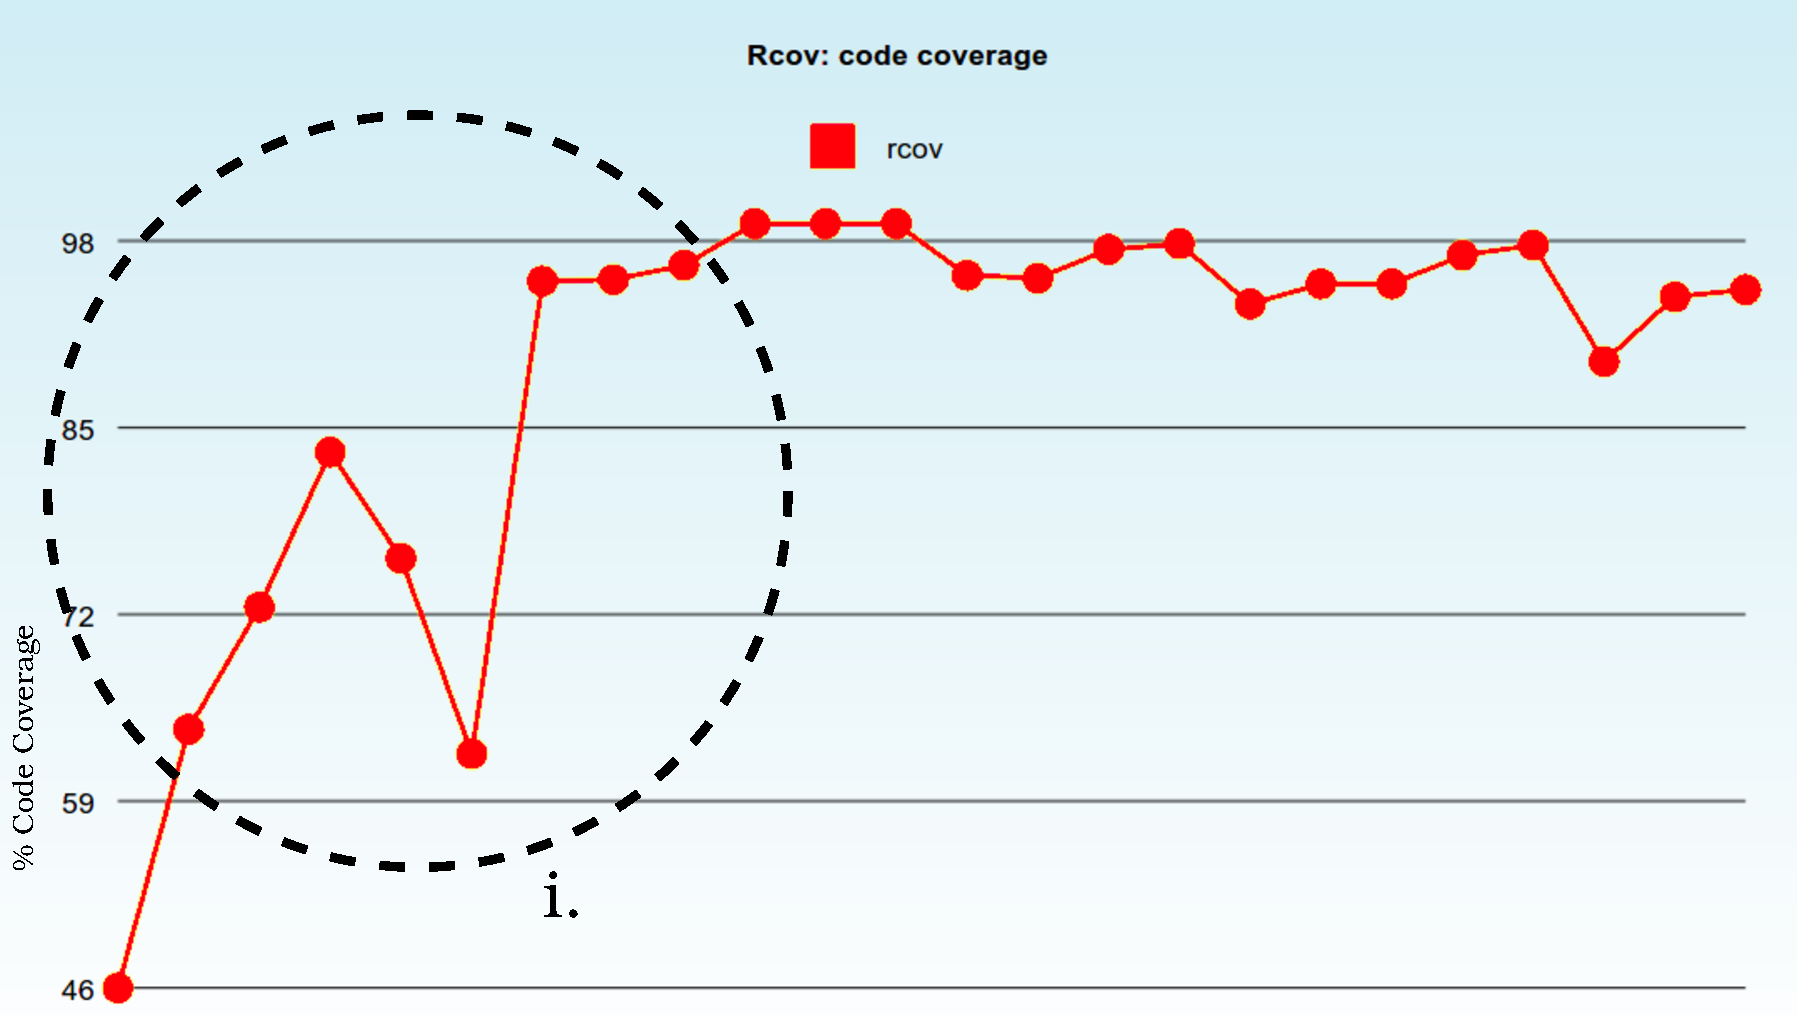
\includegraphics[width=\textwidth]{./diagrams/itjobs-coverage.pdf}
 % itjobs-coverage.pdf: 862x487 pixel, 72dpi, 30.41x17.18 cm, bb=
 \caption{C0-Testabdeckung über den Verlauf der Entwicklung}
 \label{fig:itjobsCoverage}
\end{figure}
In Abbildung \ref{fig:itjobsCoverage} ist der Verlauf der \glossar{Testabdeckung}\index{Test!Testabdeckung} über den Verlauf der Entwicklung abgebildet. Insbesondere in den ersten Tagen gab es einige Probleme, die davon verursacht wurden, dass das Tool mit dem die Abdeckung gemessen wurde, RCov nicht kompatibel mit der aktuellen Ruby Version 1.9.2 ist. RCov lieferte deshalb falsche Werte liefert. Später erfolgte eine Umstellung auf SimpleCov (bereits in Abschnitt \ref{sec:devtools} vorgestellt). Ab dann lag die Testabdeckung innerhalb von 90\% bis 100\%.

\begin{figure}[htbp]
 \centering
 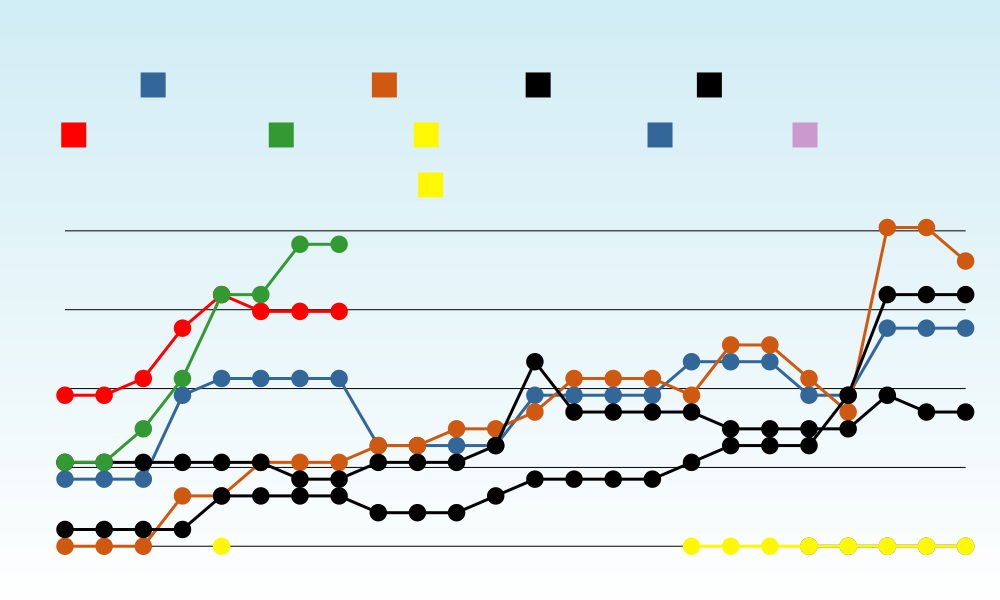
\includegraphics[width=\textwidth]{./diagrams/itjobs-smells.png}
 % itjobs-coverage.pdf: 862x487 pixel, 72dpi, 30.41x17.18 cm, bb=
 \caption{Verlauf der verschiedenen Klassen an Code-Smells über den Entwicklungszeitraum}
 \label{fig:itjobsSmells}
\end{figure}

Ein Indikator für die \glossar{quality} sind die Anzahl und Arten von Code-Smell\index{Code-Smell}s. Diese wurden ebenfalls über den Entwicklungszeitraum gemessen und sind in Abbildung \ref{fig:itjobsSmells} dargestellt. Insgesamt betrachtet, stiegen diese mit zunehmender Codemenge langsam an. Dank der Messung durch Code-Metrik\index{Code-Metrik}en konnten einige suboptimale Stellen nach einer gewissen Zeit refaktorisiert werden. So ist das wiederkehrende Muster zu erklären, dass die Anzahl der Vorkommen eines Codesmells erst anstieg und nach einigen Tagen wieder abfiel. Das Ergebnis gilt als positiv zu bewerten, da die Menge an Code-Smells langsamer anstieg, als die dazugehörige Menge an Code (LOC, vgl. Abbildung \ref{fig:itjobsLoc}). Die Code-Smells wurden mit dem Werkzeug Reek gemessen und die Definition der Code-Smells sowie Informationen über das jeweilige Messverfahren entnehmen sie bitte \citep{kevin_rutherford_code_2010}.

\subsection*{Diskussion}
Falls das Projekt in einem reinen TDD\index{TDD}-Vorgehen entwickelt worden wäre, dann hätte die Testabdeckung\index{Test!Testabdeckung} 100\% betragen müssen. Dies war aber nicht immer der Fall. Gründe hierfür sind:
\begin{description}
 \item[Nutzung von Codegeneratoren]\index{Code-Generato} Bei der Erstellung der Gerüste und der Programmierung einfacher Administrationsinterfaces waren nicht immer Testfälle mitgeneriert worden. Stellenweise wurde dieser generierte Code später neu in TDD\index{TDD} geschrieben, allerdings nicht in allen Fällen
 \item[Erfahrungsgewinn mit Rails] Vorher waren schon einige Erfahrung mit Rails\index{Ruby-on-Rails} vorhanden. Allerdings sind in der neusten Version von Rails einige Features dazu gekommen und wurden nun einige Bibliotheken verwendet, die vorher noch nicht bekannt waren. Aus der Unkenntnis entstand so viel Code, der eigentlich zum Experimentieren mit diesen neuen Features gedacht war. Diese Spikes (siehe Abschnitt \ref{sec:tddspecialcircumstances}) dienen dem Erkunden neuer Funktionalitäten und dem Prototypisieren. Diese sollten normalerweise nicht in den Hauptzweig der Entwicklung mit eingecheckt werden. In zukünftigen Projekten, die nach dem Prinzip der kontinuierlichen Integration stattfinden werden (siehe Abschnitt \ref{sec:auswahlWeitere}), wird ein Einchecken dieser Spikephasen in den Hauptzweig der Entwicklung nicht erfolgen.
 \item[Erfahrungsgewinn mit TDD] Trotz bisheriger Erfahrungen mit Ruby und Rails\index{Ruby-on-Rails} waren nur wenig Erfahrungen zum Thema Testen und Testgetriebene\index{TDD} Entwicklung vorhanden. Insbesondere die Nutzung von \glossarpl{Test-Double}\index{Test-Double} musste erst gelernt werden, da ohne diese bestimmte Testszenarien schwierig bis überhaupt nicht zu testen sind.
\end{description}

Trotzdem ermöglichte die vorhandene Testdichte eine sichere Ausgangsbasis für ständige Refaktorisierung\index{Refaktorisierung}en. Ein Ergebnis dessen ist, dass die Anzahl der Code-Smell\index{Code-Smell}s im akzeptablen Rahmen geblieben ist. Eine gewisse Menge an Komplexität lässt sich nicht vermeiden und Code-Smells können hier nur ein Indikator sein. In vielen Fällen muss direkt am Code entschieden werden, ob ein spezifischer Code-Smell für eine gewisse Quelltextstelle relevant ist oder nicht.

\section{Code-Quality-Benchmark mit anderen Ruby-Projekten}
\label{sec:benchmarkAll}

Um die Ergebnisse besser einordnen zu können, vergleichen wir die Ergebnisse aus den Code-Quality-Benchmarks mit vergangenen Ruby\index{Ruby}-Projekten in der pludoni GmbH und mit bekannten Ruby/Rails\index{Ruby-on-Rails}-OpenSource-Applikationen und -Bibliotheken.

Eine vollständige Metrik wie oben an IT-Jobs\index{IT-Jobs-Projekt} war in vielen Fällen nicht möglich, da die Testwerkzeuge in vielen Fällen Inkompatibilitäten mit neueren Rubyversionen haben. Wir beschränken uns deshalb auf eine exemplarische Überblicksmetrik, bestehend aus:

\begin{description}
 \item[LOC] Anzahl der Quellcodezeilen, gemessen durch das \glossar{rake}-Tasks \texttt{rake stats}\index{Ruby!Rake}.
 \item[LOT] Anzahl der Quellcodezeilen aller Tests, ebenfalls gemessen durch das Rails-Kommando \texttt{rake stats}.
 \item[LOT/TOC] Verhältnis aus Testzeilen und Quellcodezeilen.
 \item[AVGCmplx] Durchschnittliche Komplexität aller Klassen, gemessen durch \textbf{Flog}\footnote{\url{https://github.com/seattlerb/flog}}. Flog besitzt ein eigenes Maß für Code-Komplexität. Es vergibt für jede Zuweisung, Verzweigung und Funktionsaufruf unterschiedlich viele Punkte und bildet so eine Summe je Funktion oder je Klasse. Dabei vergibt Flog besonders viele Punkte für schwer nachzuvollziehende Funktionsaufrufe, wie z.B. \texttt{eval(string)}, welches einen String als Ruby\index{Ruby}-Code auswertet.
 \item[H5Cmplx] Komplexität oberen 5\% komplexesten Klassen (mindestens 1 Klasse), nach Flog.
 \item[DSmell] Anzahl der Code Smells nach \textbf{Roodi}\footnote{\url{https://github.com/martinjandrews/roodi}}. Beinhaltet u.a.: hohe zyklomatische Komplexität in einer Methode (min. 4), lange Methoden, lange Parameterlisten, u.v.m.\footnote{\url{http://roodi.rubyforge.org/files/README_txt.html}}
 \item[DSmell/KLOC] Anzahl der Code Smells nach Roodi pro tausend Codezeilen.
 \item[CSmell] Anzahl der Code Smells nach Reek. Diese beinhalten: geringe Kohäsion, Duplikation, unkommunikativer Name von Methoden/Variablen/Parameter, verschachtelte Iteratoren, u.v.m.\footnote{\url{https://github.com/kevinrutherford/reek/wiki/Code-Smells}} (vgl. Abschnitt \ref{sec:smells}).
 \item[CSmell/KLOC] Anzahl der Code Smells nach Reek pro tausend Codezeilen.
\end{description}







\subsection{Vergleich von IT-Jobs mit eigenen Projekten}

Bisherige Projekte der pludoni GmbH und des Autors basierend auf Ruby\index{Ruby}/ Ruby on Rails\index{Ruby-on-Rails}:
\begin{description}
 \item[feedimport] Die fertiggestellte Bibliothek zum Parsen und Import von Stellenanzeigen, die im Rahmen der Entwicklung von IT-Jobs\index{IT-Jobs-Projekt} ausgelagert wurde, um den Community-Portalen bereits jetzt zur Verfügung zu stehen. Die Grundzüge wurden in Abschnitt \ref{sec:awmock} vorgestellt.
 \item[feedmerger] Eine Rails\index{Ruby-on-Rails}-Anwendung\footnote{ Als OpenSource unter \url{https://github.com/zealot128/WenShanWenHai} zu finden.} zur Verwaltung, Cachen, Filtern und Zusammenfügen von RSS- und Atom-Feeds.
 \item[pludonidb] Eine auf ActiveRecord\index{ActiveRecord} basierende Bibliothek zur Anbindung der Datenbank\index{Datenbank}en der Communityportale an Ruby-Skripte. Beinhaltet außerdem weitere Hilfsfunktionen für Berechnung von Tag-Wolken, Häufigkeiten u.ä.
 \item[backlinks] Backlink und SEO-Success-Control ist eine Rails-2.3 Anwendung zum Messen der sogenannten Backlinks\footnote{Backlinks sind Links anderer Webseiten auf die Eigene. In den Communityportalen sind die Mitglieder vertraglich verpflichtet, einen Backlink auf die Communityportale anzulegen.} der Communitymitglieder und der Platzierung für relevante Sucheingaben in den großen Suchmaschinen (konkret: Welchen Platz hatte ein Communityportal an einem bestimmten Tag für einen konkreten Suchbegriff). Details dazu sind im Praktikumsbericht des Autors zu finden. %TODO Verweis auf meinen Praktikumsbericht

 \item[SiteAnalyzer (SAnalyzer)] Ein Werkzeuge zur Analyse von kompletten Websites/Webdomains mit dem Ziel, tote Links zu finden, alle Seiten auf HTML-Gültigkeit zu prüfen und insgesamt die Link-Architektur zu analysieren\footnote{Auch dieses Projekt ist als OpenSource verfügbar: \url{https://github.com/zealot128/Site-Structure-Analyzer}}.
\end{description}


\begin{table}[hbp]
  \caption{Vergleich von IT-jobs mit anderen Ruby Projekten des Autors/der pludoni GmbH}\label{table:cmpmy}
  \begin{center}
    \begin{tabular}{|l|l|l|l|l|l|l|}
      \hline\rowcolor{tableheadcolor}

      Projekt&ItJobs&Backlinks&Feedmerger&SAnalyzer&Feedimport&PludoniDb\\
      \hline
      Technologie&Rails3&Rails2&Rails3&Rails3&Ruby&Ruby\\
      \hline
      Testverfahren&TDD&manuell&manuell&manuell&TDD&manuell\\
      \hline
      LOC&1570&1884&724&214&571&1933\\
      \hline
      LOT&1750&75&137&0&865&126\\
      \hline
      LOT/LOC&1.11&0.04&0.19&0.00&1.51&0.07\\
      \hline
      AVGCmplx&8.00&19.90&10.50&14.80&16.80&13.70\\
      \hline
      H5Cmplx&43.80&70.60&26.90&39.70&25.10&113.20\\
      \hline
      DSemll&11&69&11&11&8&25\\
      \hline
      DSmell/KLOC&7.00&36.60&15.20&51.40&14.00&12.90\\
      \hline
      CSmell&53&152&52&13&28&113\\
      \hline
      CSmell/KLOC&33.80&80.70&71.80&60.70&49.00&58.50\\
      \hline
    \end{tabular}
  \end{center}

\end{table}


\subsection{Vergleich von IT-Jobs mit anderen Rails-Projekten}
Weiterhin wird das Projekt mit folgenden beliebten Webprojekten, welche ebenfalls auf Ruby on Rails\index{Ruby-on-Rails} basieren, verglichen:
\begin{description}
\item[lpp] Das Linkpartnerprogramm ist eine Studenteninitiative der TU Dresden, um ausländische Studenten mit deutschen Sprach- und Lernpartnern zusammenzubringen. Dazu wurde 2008 von einem Studententeam im Rahmen einer Semesterarbeit eine Rails\index{Ruby-on-Rails}-Webanwendung geschrieben, die unter \url{http://linkpartnerprogramm.de} zu finden ist. Der Autor dieser Arbeit war zwar nicht an der Entwicklung beteiligt, übernahm aber die Pflege und Weiterentwicklung selbiger.
 \item[diaspora] Ein verteiltes soziales Netzwerk (vgl. Google+ und Facebook) \\
 Code: \url{https://github.com/diaspora/diaspora}
 \item[bucketwise (bucket)] Ein Web-basierter persönlicher Finanzmanager mit Budgetierung nach dem Briefumschlagsystem.\\
 Code: \url{https://github.com/jamis/bucketwise}
 \item[chiliproject (chilli)] Ein Fork\footnote{In der (Open-Source)-Software-Entwicklung ist ein Fork eine legale Kopie eines bestehendes Software-Produktes, um von nun an eine unabhängige Entwicklung zu betreiben.} des sehr beliebten Bugtrackers Redmine\footnote{https://github.com/edavis10/redmine}. Statt des originalen Redmines wurde dieser Fork verwendet, da er eine neuere Codebasis hat.\\
 Code: \url{https://github.com/chiliproject/chiliproject}
 \item[railscast (rCasts)] Der Code der Website \url{http://www.railscasts.com}, in welche allwöchentlich ein Screencast zum Thema Ruby und Rails veröffentlich wird (bis dato 283 Episoden).\\
 Code: \url{https://github.com/ryanb/railscasts}
 \item[ActiveSupport (aSupport)] Beinhaltet Hilfsklassen und Erweiterungen der Ruby\hyp{}Standardbibliothek und ist Kernbestandteil von Ruby on Rails. \\
 Code: \url{https://github.com/rails/rails.git}
 \item[ActionPack (aPack)] Ein Framework, um Anfragen und Antworten eines Webservers zu verarbeiten und ein weiterer Kernbestandteil von Rails.\\
 Code: \url{https://github.com/rails/rails.git}
\end{description}

Die Auswahl erfolgt z.T. willkürlich. Als Ansatzpunkt diente die Liste der beliebtesten Rails\index{Ruby-on-Rails}-Projekte, die auf Github gehostet sind\footnote{\url{https://github.com/search?q=rails&type=Repositories}}. Weiterhin wurde ActiveSupport und ActionPack ausgewählt, um die Code-Qualität von Rails selbst mit zu beurteilen.

\begin{table}[hbp]
 \caption{Vergleich von IT-jobs mit Ruby/Rails Projekten aus der Community}\label{table:cmpother}
 \begin{tabular}{|p{1.8cm}|l|l|l|l|l|l|l|l|}
\hline \rowcolor{tableheadcolor}
 Projekt&itjobs&bucket&lpp&chili&aPack&aSupport&diaspora&rCasts\\
\hline
Technol.&Rails3&Rails2&Rails1&Rails2&Rails3&Rails3&Rails3&Rails3\\
\hline
LOC&1570&1979&7116&21201&12995&9407&7466&653\\
\hline
LOT&1750&1684&1557&20127&32570&13590&10072&748\\
\hline
LOT/LOC&1.11&0.85&0.22&0.95&2.51&1.44&1.35&1.15\\
\hline
AVGCmplx&8.00&12.80&17.10&19.10&11.10&10.90&13.10&11.00\\
\hline
H5Cmplx&43.80&32.20&181.80&84.40&64.00&47.90&54.00&34.60\\
\hline
DSmell&11&37&250&651&370&166&99&2\\
\hline
DSmell\newline~/KLOC&7.00&18.70&35.10&30.70&28.50&17.60&13.30&3.10\\
\hline
CSmell&53&129&386&1535&982&291&324&42\\
\hline
CSmell\newline~/KLOC&33.80&65.20&54.20&72.40&75.60&30.90&43.40&64.30\\
\hline
\end{tabular}
\end{table}

\subsection{Auswertung und Visualisierung}
\label{sec:auswertungFinal}
In den Abbildungen \ref{fig:cpm-loclot}, \ref{fig:cpm-complex} und \ref{fig:cpm-smells} werden die gesammelten Ergebnisse für alle genannten Projekte visualisiert. Der obere Teil jeder Abbildung enthält die externen Projekte, der untere alle Projekte der pludoni GmbH.
\begin{figure}[htbp]
 \centering
 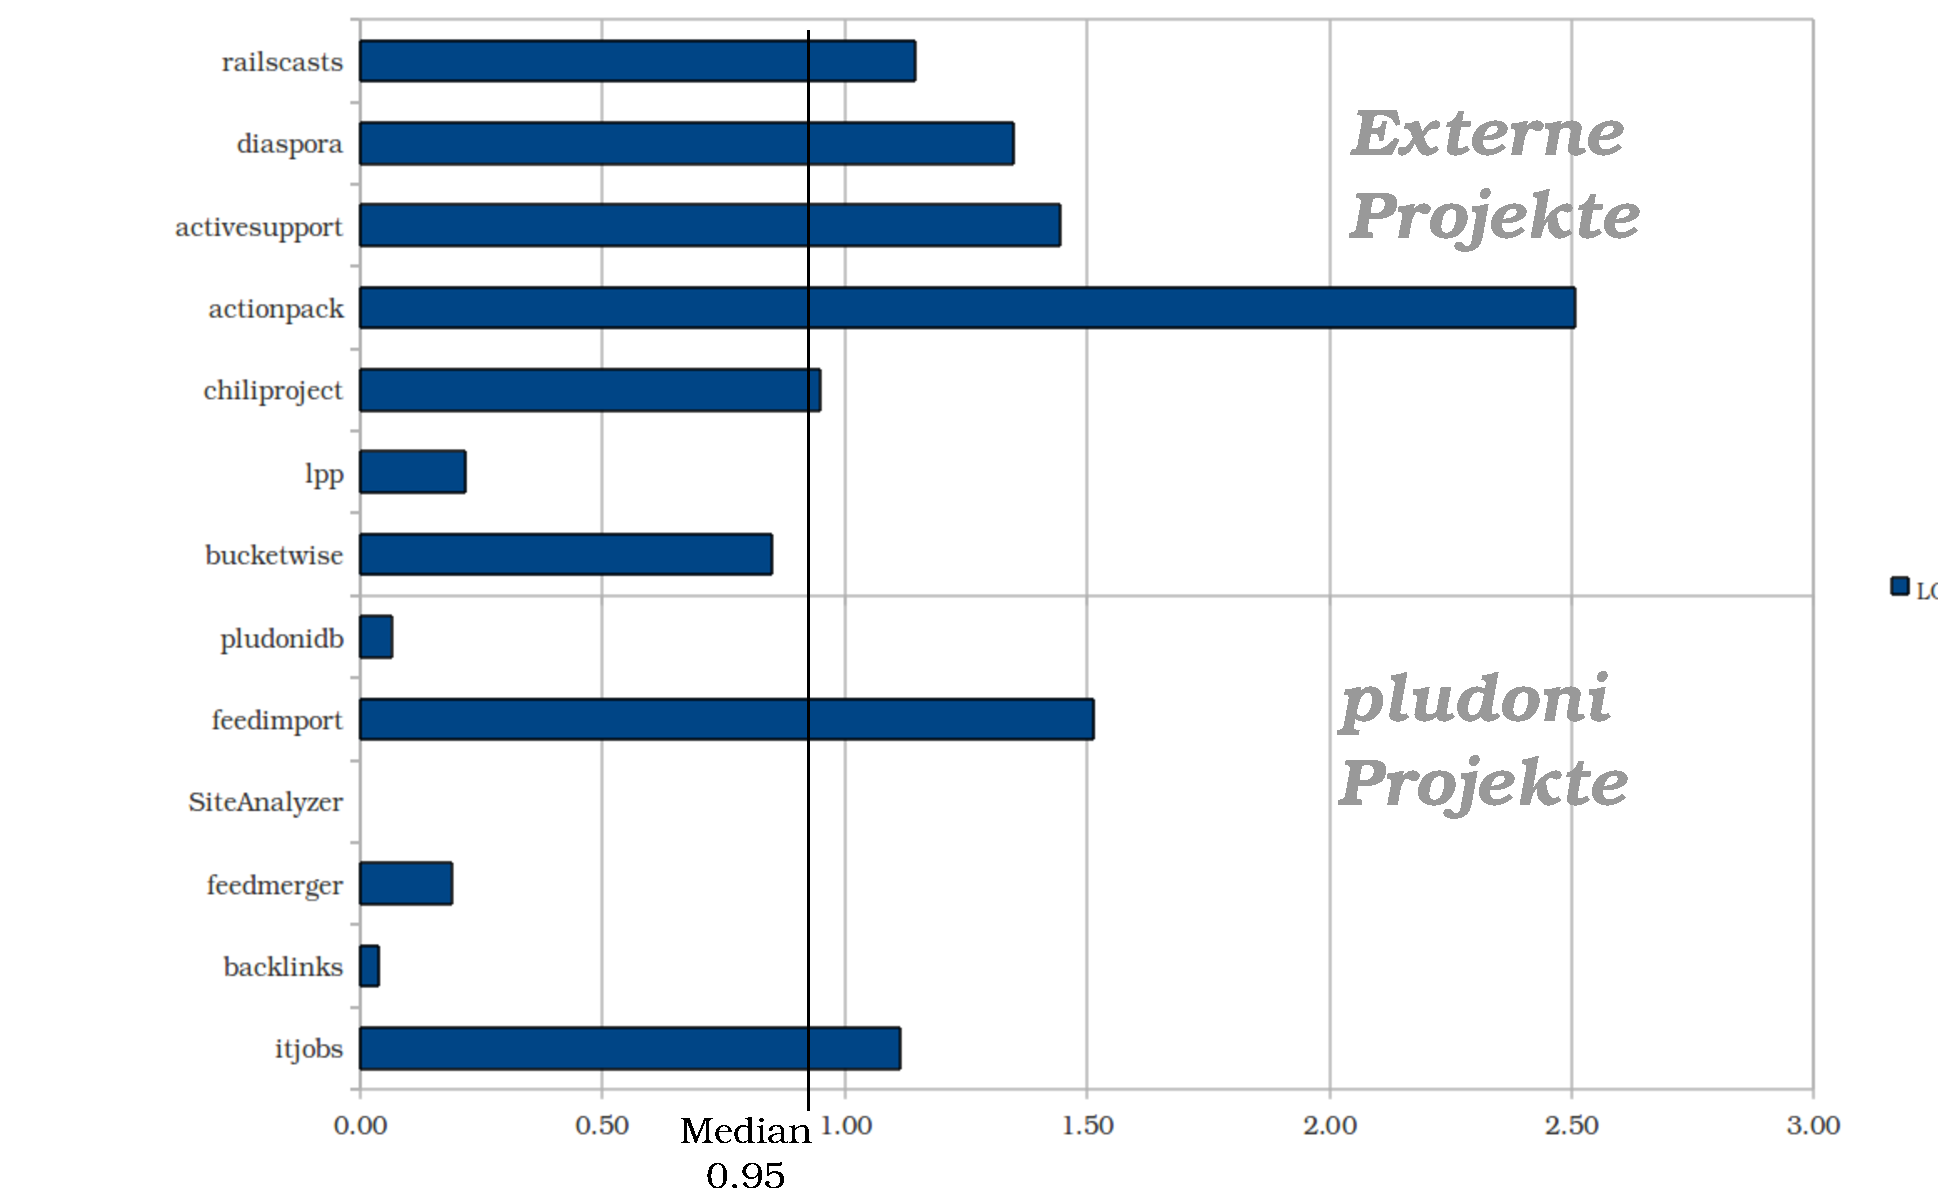
\includegraphics[width=\linewidth]{./diagrams/cpm-lotloc.pdf}
 % cpm-lotloc.pdf: 930x574 pixel, 72dpi, 32.81x20.25 cm, bb=0 0 930 574
 \caption{Vergleich des Verhältnisses aus Anzahl Testcodezeilen / Anzahl Codezeilen}
 \label{fig:cpm-loclot}
\end{figure}

Abbildung \ref{fig:cpm-loclot} zeigt das Verhältnis aus Testcode zu Programmcode. Der Median über alle Projekte ist 0.95. Ausreißer sind hierbei vier der internen Projekte pludonidb, SiteAnalyzer, feedmerger und backlinks, die wenig bis gar keine automatisierten  Tests besitzen. Als Gegenbeispiel sei ActionPack zu nennen, dass über 2.5x soviel Testcodezeilen wie Programmcode verfügt. Gegenüber den bisherigen Projekten in der pludoni GmbH kann man anhand der Projekte Feedimport und IT-Jobs\index{IT-Jobs-Projekt}, die im Rahmen dieser Diplomarbeiten entstanden sind, sehen, dass die bloße Anzahl an Tests stark zugenommen hat. Beide Projekte wurden mittels TDD\index{TDD} entwickelt. Gegenüber dem Feedimport nutzt IT-Jobs aber Rails als Grundlage. Dies bedeutet, dass dadurch viel Logik durch das Framework implementiert und vorgegeben wurde. Der Feedimport dagegen besitzt eine komplett eigene Objekthierarchie und hat darum mehr Tests benötigt als IT-Jobs.

\begin{figure}[htbp]
 \centering
 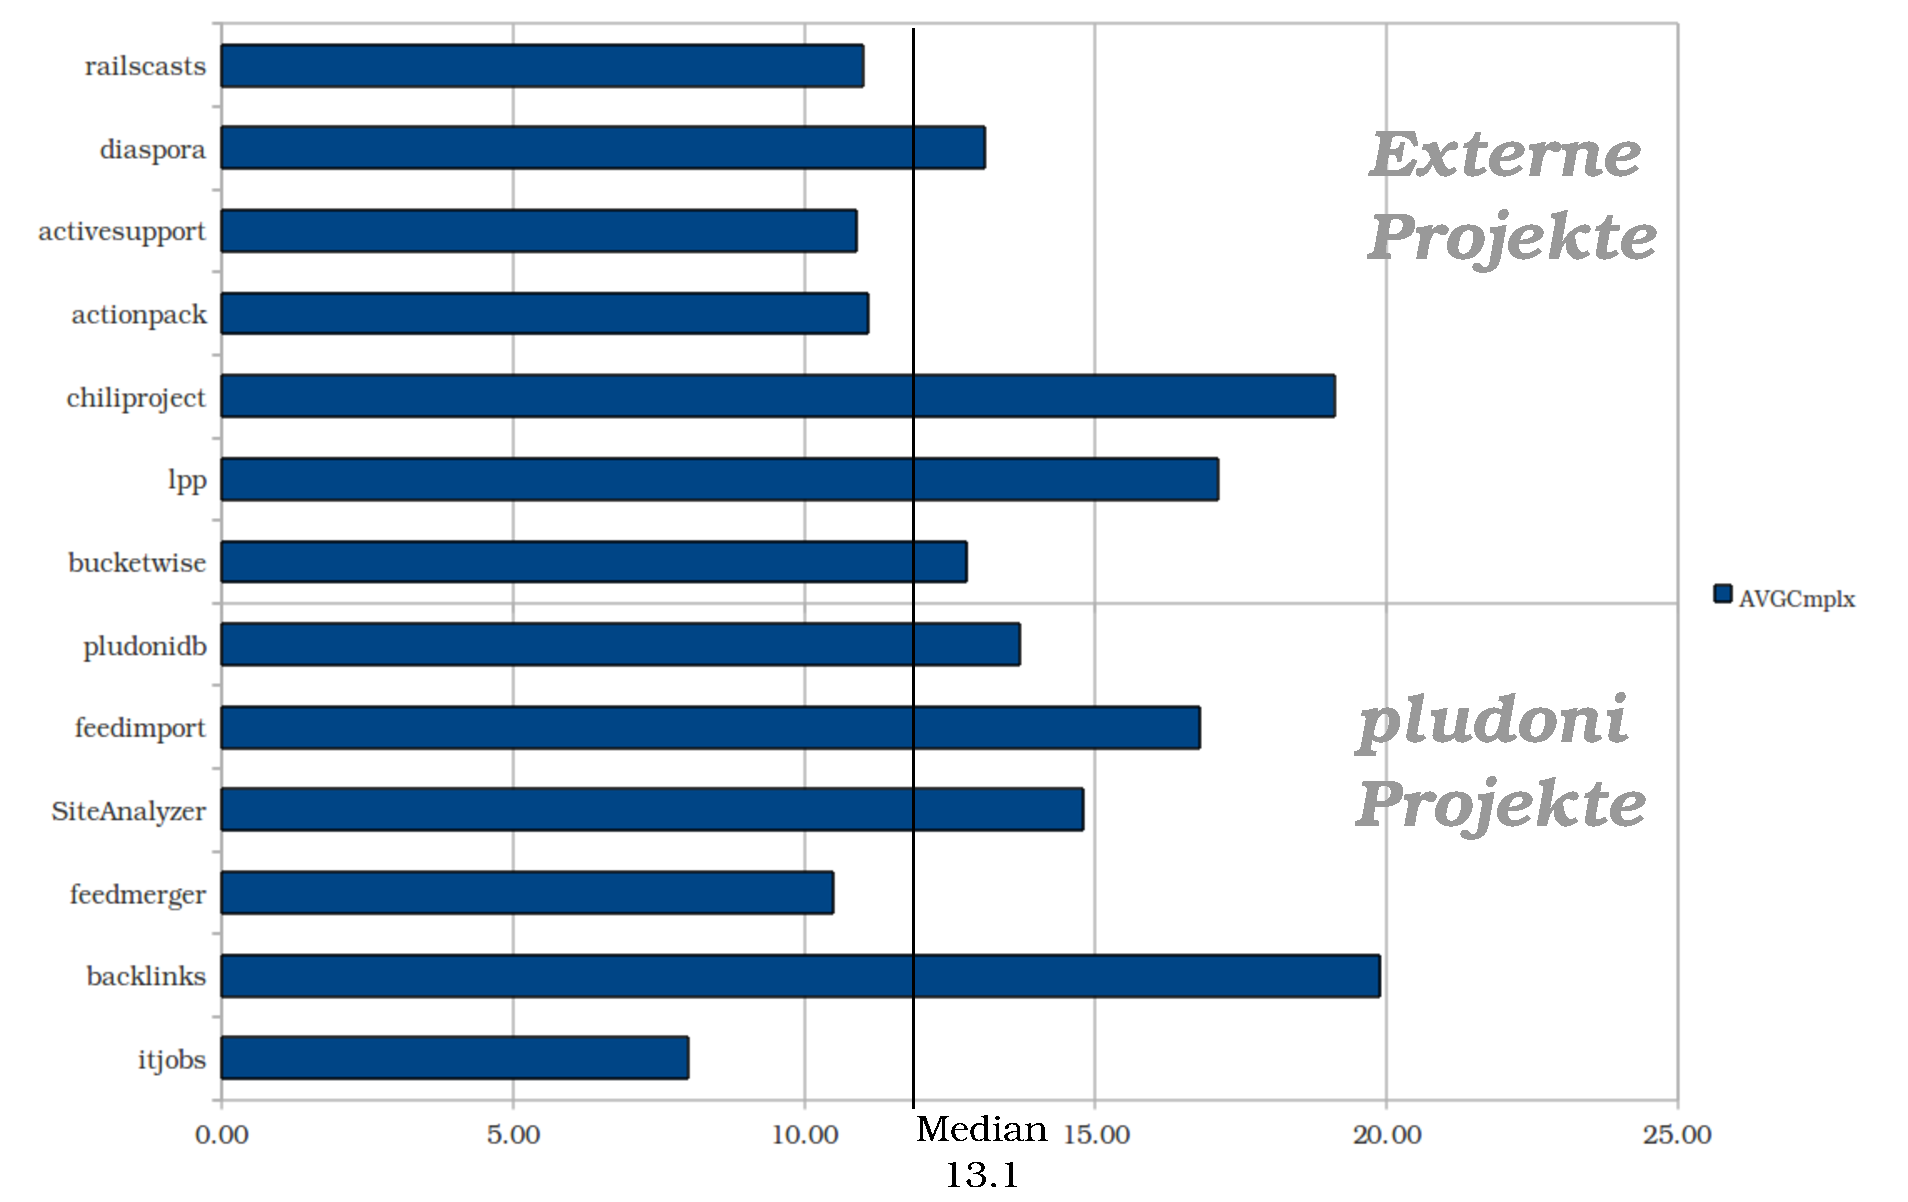
\includegraphics[width=\linewidth]{./diagrams/cmp-complex.pdf}
 % cpm-lotloc.pdf: 930x574 pixel, 72dpi, 32.81x20.25 cm, bb=0 0 930 574
 \caption{Vergleich der durchschnittlichen Komplexität}
 \label{fig:cpm-complex}
\end{figure}
In Abbildung \ref{fig:cpm-complex} wurde die durchschnittliche Komplexität nach dem Flog-Verfahren gegenübergestellt. Der Median war hier 13,1. Unter den eigenen Projekten sind hier Backlinks und der Feedimport die komplexesten Projekte. IT-Jobs\index{IT-Jobs-Projekt} und Feedmerger, die beide Rails-Projekte sind, haben dagegen eine geringere Code-Komplexität. Die Ursache ist hier, dass während der Entwicklung von IT-Jobs ständig die Code-Qualität durch die Metriken gemessen wurde und im Falle von Ausreißern gegengesteuert wurde. Bei dem Feedimport, der ebenfalls durch TDD\index{TDD} entwickelt wurde, wurde eine solche Analyse erst am Ende der Entwicklung durchgeführt. Für uns ist das ein Indiz, dass die Nutzung einer Testgetriebenen Entwicklung kein alleiniger Garant für eine gute Code-Qualität ist.\\
Bei den externen Projekten war die Bugtracker-Anwendung Chiliproject/Redmine das komplexeste Projekt, dicht gefolgt von der Sprachpartnervermittlung Linkpartnerprogramm. Gerade wenn man das Verhältnis aus Testcode zu Programmcode mit einbezieht, kann man eine Tendenz ableiten: beide Projekte haben gegenüber den anderen Externen eine relativ geringe Anzahl an Testcode und beide haben eine relativ hohe Komplexität.

\begin{figure}[htbp]
 \centering
 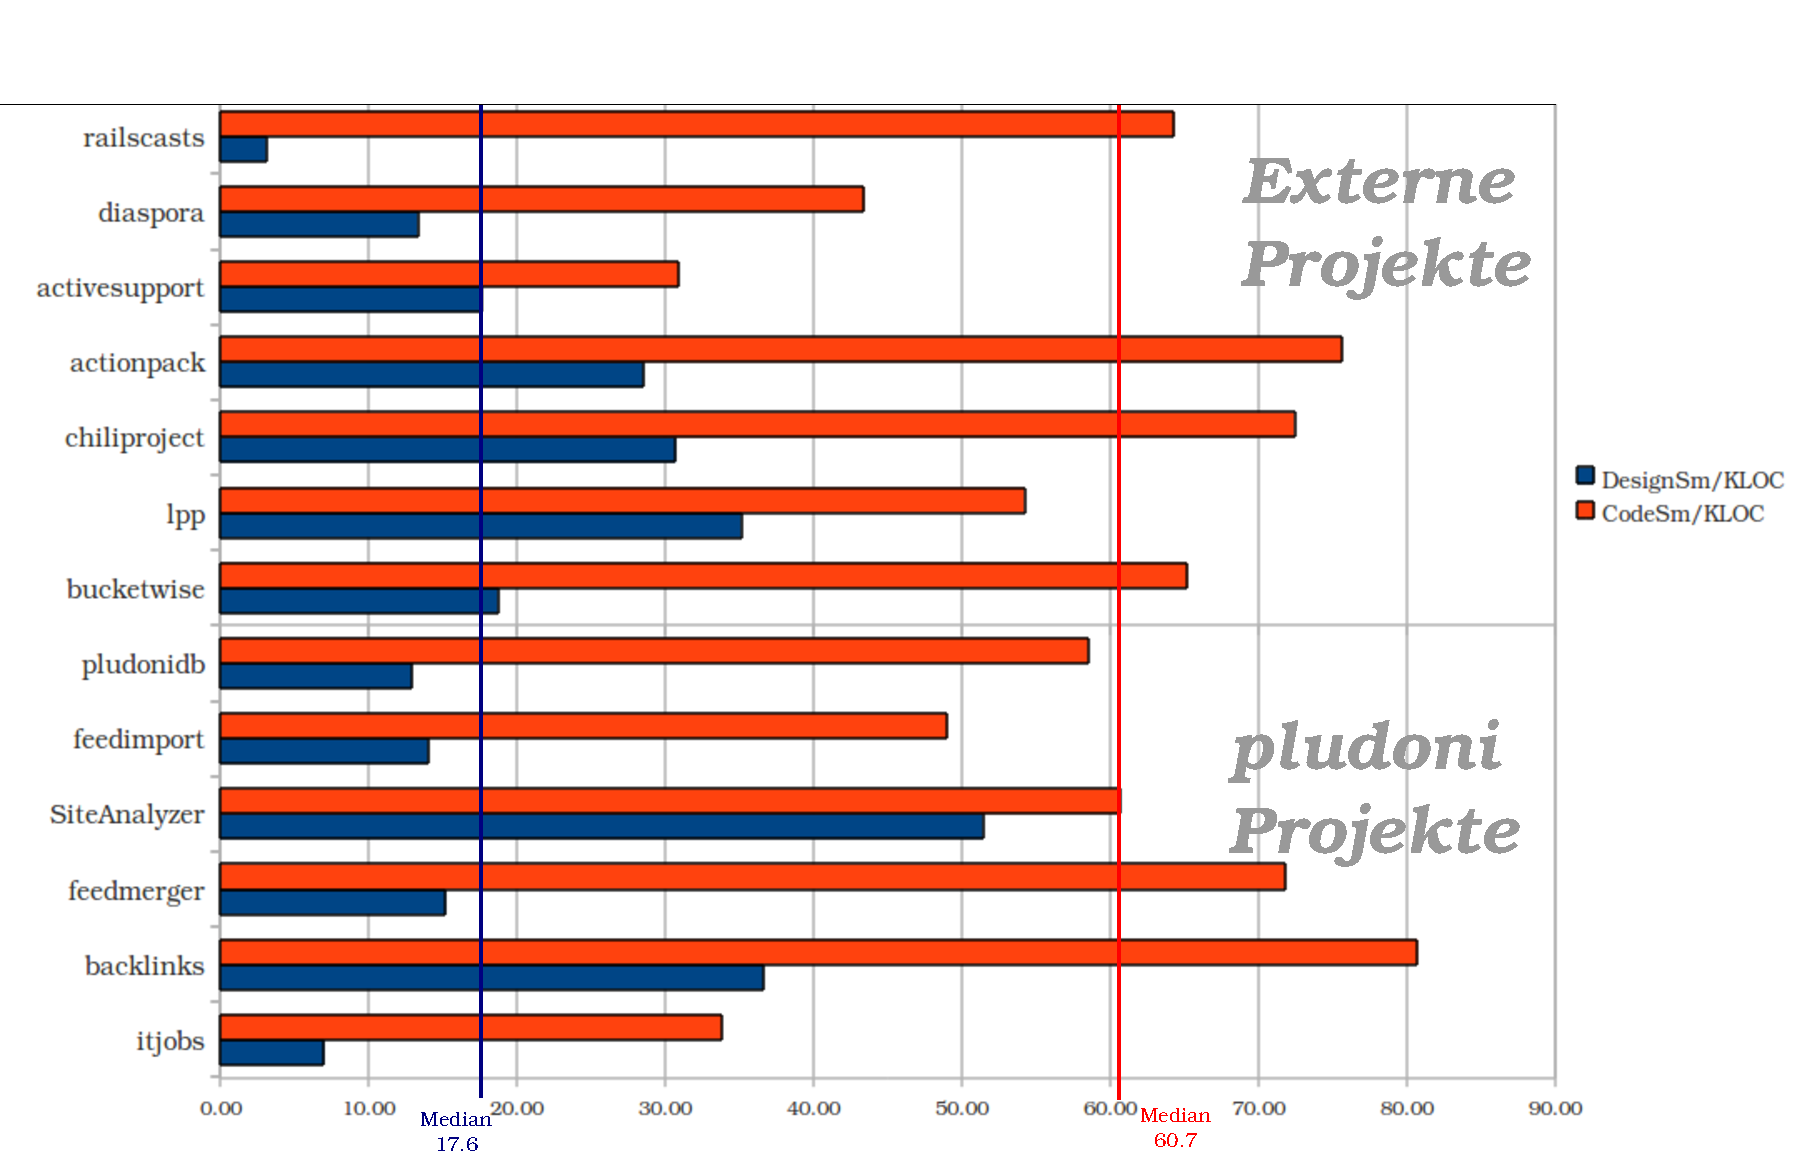
\includegraphics[width=\linewidth]{./diagrams/cpm-smells.pdf}
 % cpm-lotloc.pdf: 930x574 pixel, 72dpi, 32.81x20.25 cm, bb=0 0 930 574
 \caption{Vergleich der Anzahl Smells pro KLOC}
 \label{fig:cpm-smells}
\end{figure}
Die Abbildung \ref{fig:cpm-smells} zeigt zwei verschiedene Arten von Smell\index{Code-Smell}s: einerseits durch Reek gemessen (Rot) und andererseits durch Roodi gemessen (Blau). Zu bemerken ist, dass IT-Jobs\index{IT-Jobs-Projekt} eine deutlich geringere Code-Smell-Dichte (1/2 Median) besitzt. Auch der Feedimport ist noch im Rahmen und leicht unter dem Schnitt. Dagegen hat das interne Projekt Backlinks die höchste Dichte an Code Smells. Interessanterweise hat dieses Projekt auch so gut wie gar keine automatisierten Tests, was eine nachträgliche Refaktorisierung\index{Refaktorisierung} sehr erschwert. Für das Projekt Feedimport existiert allerdings eine gute Testabdeckung\index{Test!Testabdeckung} und so ließen sich leicht weitere Refaktorisierungen durchführen, sollte das gewünscht sein. \\
Actionpack weist trotz der großen Menge an Tests und der relativ geringen Komplexität unter den externen Projekten die höchste Smell\index{Code-Smell}-Dichte auf. Da Actionpack auch das umfangreichste Projekt unter den Untersuchten ist, läge hier ein guter Ansatzpunkt für weitere Untersuchungen in der Sinnhaftigkeit gewisser Code-Smells. \\
Die mit Abstand häufigsten Code-Smells hierbei waren geringe Kohäsion bzw. starke Kopplung unter den Klassen. Eventuell lassen sich einige der Smells bei großen Modulen nicht vermeiden, da diese zwangsweise untereinander gekoppelt sein müssen.

Für \randbem{Schlussfolgerung}statistisch signifikante Ergebnisse reichen die hier präsentierten Daten nicht aus, stattdessen sollte nur eine Tendenz untersucht werden. Insbesondere der Vergleich mit den internen Projekten hinsichtlich Code-Qualität ist für weitere Projektplanungen interessant. Das Gefühl der Programmierer, dass z.B. das Projekt Backlinks eine relativ schlechte Codebasis verfügt, wurde durch die hier gezeigten Metriken bestätigt. Der aktuelle Stand von IT-Jobs\index{IT-Jobs-Projekt} dagegen lässt eine gute Ausgangsbasis für eine Weiterentwicklung vermuten.







